\documentclass[english,floatsintext,man]{apa6}

\usepackage{amssymb,amsmath}
\usepackage{ifxetex,ifluatex}
\usepackage{fixltx2e} % provides \textsubscript
\ifnum 0\ifxetex 1\fi\ifluatex 1\fi=0 % if pdftex
  \usepackage[T1]{fontenc}
  \usepackage[utf8]{inputenc}
\else % if luatex or xelatex
  \ifxetex
    \usepackage{mathspec}
    \usepackage{xltxtra,xunicode}
  \else
    \usepackage{fontspec}
  \fi
  \defaultfontfeatures{Mapping=tex-text,Scale=MatchLowercase}
  \newcommand{\euro}{€}
\fi
% use upquote if available, for straight quotes in verbatim environments
\IfFileExists{upquote.sty}{\usepackage{upquote}}{}
% use microtype if available
\IfFileExists{microtype.sty}{\usepackage{microtype}}{}

% Table formatting
\usepackage{longtable, booktabs}
\usepackage{lscape}
% \usepackage[counterclockwise]{rotating}   % Landscape page setup for large tables
\usepackage{multirow}		% Table styling
\usepackage{tabularx}		% Control Column width
\usepackage[flushleft]{threeparttable}	% Allows for three part tables with a specified notes section
\usepackage{threeparttablex}            % Lets threeparttable work with longtable

% Create new environments so endfloat can handle them
% \newenvironment{ltable}
%   {\begin{landscape}\begin{center}\begin{threeparttable}}
%   {\end{threeparttable}\end{center}\end{landscape}}

\newenvironment{lltable}
  {\begin{landscape}\begin{center}\begin{ThreePartTable}}
  {\end{ThreePartTable}\end{center}\end{landscape}}




% The following enables adjusting longtable caption width to table width
% Solution found at http://golatex.de/longtable-mit-caption-so-breit-wie-die-tabelle-t15767.html
\makeatletter
\newcommand\LastLTentrywidth{1em}
\newlength\longtablewidth
\setlength{\longtablewidth}{1in}
\newcommand\getlongtablewidth{%
 \begingroup
  \ifcsname LT@\roman{LT@tables}\endcsname
  \global\longtablewidth=0pt
  \renewcommand\LT@entry[2]{\global\advance\longtablewidth by ##2\relax\gdef\LastLTentrywidth{##2}}%
  \@nameuse{LT@\roman{LT@tables}}%
  \fi
\endgroup}


\ifxetex
  \usepackage[setpagesize=false, % page size defined by xetex
              unicode=false, % unicode breaks when used with xetex
              xetex]{hyperref}
\else
  \usepackage[unicode=true]{hyperref}
\fi
\hypersetup{breaklinks=true,
            pdfauthor={},
            pdftitle={Moos as cues: One-to-one biases in a non-linguistic and non-communicative domain},
            colorlinks=true,
            citecolor=blue,
            urlcolor=blue,
            linkcolor=black,
            pdfborder={0 0 0}}
\urlstyle{same}  % don't use monospace font for urls

\setlength{\parindent}{0pt}
%\setlength{\parskip}{0pt plus 0pt minus 0pt}

\setlength{\emergencystretch}{3em}  % prevent overfull lines

\ifxetex
  \usepackage{polyglossia}
  \setmainlanguage{}
\else
  \usepackage[english]{babel}
\fi

% Manuscript styling
\captionsetup{font=singlespacing,justification=justified}
\usepackage{csquotes}
\usepackage{upgreek}



\usepackage{tikz} % Variable definition to generate author note

% fix for \tightlist problem in pandoc 1.14
\providecommand{\tightlist}{%
  \setlength{\itemsep}{0pt}\setlength{\parskip}{0pt}}

% Essential manuscript parts
  \title{Moos as cues: One-to-one biases in a non-linguistic and
non-communicative domain}

  \shorttitle{Moos as cues}


  \author{Kyle MacDonald\textsuperscript{1}, Ricardo A. H. Bion\textsuperscript{1}, Virginia A. Marchman\textsuperscript{1}, \& Anne Fernald\textsuperscript{1}}

  \def\affdep{{"", "", "", ""}}%
  \def\affcity{{"", "", "", ""}}%

  \affiliation{
    \vspace{0.5cm}
          \textsuperscript{1} Stanford University  }

 % If no author_note is defined give only author information if available
      \newcounter{author}
                              \authornote{
            Correspondence concerning this article should be addressed to Kyle MacDonald, 450 Serra Mall, Stanford, CA 94306. E-mail: \href{mailto:kylem4@stanford.edu}{\nolinkurl{kylem4@stanford.edu}}
          }
                                                              

  \abstract{When hearing a novel name, children tend to select a novel object rather
than a familiar one, a bias known as disambiguation. This bias is often
assumed to reflect children's expectations about the nature of words or
expectations about the communicative intention of speakers. This work
investigated whether similar biases emerge in a domain that is
non-linguistic and non-communicative for children, but in which strong
regularities can be found: the vocalizations that animals produce. Using
online processing measures, we first show that two-year-olds can
identify familiar animals based on their vocalizations, though not as
fast as they are to identify these same animals when hearing their
names. We then show that children rapidly look at an unfamiliar animal
when hearing a novel animal vocalization or novel animal name, being
equally fast in both conditions. In a follow-up experiment, we replicate
the key finding that children look at a novel animal when hearing a
novel animal vocalization, but show that these biases do not necessarily
lead to learning. We characterize disambiguation biases as resulting
from domain-general processing mechanisms, rather than from lexical or
communicative constraints.}
  \keywords{disambiguation, mutual exclusivity, environmental sounds, retention,
word learning \\

    \indent Word count: X
  }





\usepackage{amsthm}
\newtheorem{theorem}{Theorem}
\newtheorem{lemma}{Lemma}
\theoremstyle{definition}
\newtheorem{definition}{Definition}
\newtheorem{corollary}{Corollary}
\newtheorem{proposition}{Proposition}
\theoremstyle{definition}
\newtheorem{example}{Example}
\theoremstyle{definition}
\newtheorem{exercise}{Exercise}
\theoremstyle{remark}
\newtheorem*{remark}{Remark}
\newtheorem*{solution}{Solution}
\begin{document}

\maketitle

\setcounter{secnumdepth}{0}



\section{Introduction}\label{introduction}

When children encounter people and animals in daily life, they
experience them through multiple sensory modalities simultaneously. When
playing with pets, for example, the child learns to associate the
physical features and actions of dogs and cows with the barking or
mooing sounds typically produced by these animals. Eventually, the child
will also link specific spoken words to each type of animal, learning
that they are associated with the object names dog or cow, as well as
with onomatopoeic words resembling their characteristic vocalizations,
such as woof-woof or mooo. Thus, just as familiar object names,
including animal names, are consistently associated with particular
kinds of animate and inanimate objects, animal vocalizations and
onomatopoeic words for vocalizations also provide consistent
associations between auditory stimuli and different types of animal. In
this study, we compare young children's efficiency in using these
different classes of sounds as cues to identifying particular animals.
In addition, we investigate whether children can use disambiguation
strategies, which have frequently been characterized as pragmatic or
lexically-specific in nature (Bloom, 2002; Diesendruck \& Markson, 2001;
Markman, 1991) in order to infer which of two animals is associated with
a novel vocalization.

The question of whether words are a special kind of stimulus for infants
is not new. Several studies have found advantages for speech sounds over
tones in object individuation and categorization in young infants
(Fulkerson \& Waxman, 2007; Xu, 2002). Focusing on associations between
objects and sounds, objects and tones, or objects and gestures, several
studies found that younger infants accept several different forms as
potential object labels, but that older infants seem to be more
discriminating and favor words (Namy \& Waxman, 1998; Woodward \& Hoyne,
1999). A different line of research found that infants prefer to hear
spoken words over some non-linguistic analogues (Vouloumanos \& Werker,
2004, 2007a, 2007b), and that the neonate brain responds differently to
speech as compared to backwards speech (Pena et al., 2003). These
studies found advantages for speech over non-linguistic analogues in
categorization, individuation, crossmodal association, and speech
preferences. However, they all focused on arbitrary non-linguistic cues
that are not consistently associated to objects in children's everyday
environments.

Other research has approached the question of whether speech is special
from a different perspective, comparing how children process spoken
words as compared to non-arbitrary environmental sounds, such as animal
vocalizations (e.g., cat meowing) or the sounds produced by inanimate
objects (e.g., car starting). Studies with adults found similarities and
differences in both behavioral and neural responses to cross-modal
semantic associations between words and environmental sounds. In a
picture detection task, Chen and Spence (2011) found priming from
environmental sounds but not from words. These authors propose that
recognition of environmental sounds is faster because words must also be
processed at a lexical stage, while environmental sounds activate
semantic representations directly. In contrast, in a task in which
participants had to decide whether a sound and picture matched, Lupyan
and Thompson-Schill (2012) found advantages for words as compared to
environmental sounds. This finding was interpreted as evidence that
words activate conceptual information more quickly and accurately and in
a more categorical way than nonverbal sounds.

In an ERP imaging study with adults, A Cummings et al. (2006) looked at
semantic integration of verbal and non-verbal sounds and objects, and
found that largely overlapping neural networks processed verbal and
non-verbal meaningful sounds. In another study focusing on three
different sound types that varied in arbitrariness, Hashimoto et al.
(2006) found different neural mechanisms for the processing of animal
names and vocalizations, with onomatopoeic words activating both areas.
Because research on environmental sounds is still just beginning, it is
hard to reconcile these somewhat discrepant findings. Variations in
tasks or timing of stimuli can influence results, and different
theoretical commitments can lead to different interpretations. For
example, environmental sounds are often treated as encompassing both the
sounds of living and man-made objects (e.g.~cow mooing, bell ringing)
despite evidence that these sounds are treated differently by the adult
brain (Murray, Camen, Andino, Bovet, \& Clarke, 2006). But this line of
research provides promising new ways to examine the question of whether
language emerges from the interaction of domain-general cognitive
processes or domain-specific mechanism (Bates, MacWhinney, \& others,
1989). For example, recent research comparing processing of speech and
non-speech sounds is leading to new insights relevant to autism,
developmental language impairment, and cochlear implants (Alycia
Cummings \& Ceponiene, 2010; McCleery et al., 2010).

From a developmental perspective, it is also important to understand how
children process words and non-arbitrary non-linguistic sounds. Very few
studies have looked at this question. In a study using a
preferential-looking paradigm, Alycia Cummings, Saygin, Bates, and Dick
(2009) found that 15- and 25-mo-olds can use words and environmental
sounds to guide their attention to familiar objects, improving as they
get older. Vouloumanos, Druhen, Hauser, and Huizink (2009) found that
5-month-olds can match some animals to the vocalizations they produce.
And studies with children with autism and developmental language
impairment found more severe deficits for the processing of words than
environmental sounds (Alycia Cummings \& Ceponiene, 2010; McCleery et
al., 2010).

We build on these earlier studies using the looking-while-listening
paradigm, which has been widely used to assess real-time interpretation
of spoken words by infants and young children (Fernald, Pinto, Swingley,
Weinbergy, \& McRoberts, 1998; Fernald, Zangl, Portillo, \& Marchman,
2008). One major goal in this research is to investigate how
two-year-old children process different types of auditory stimuli that
are consistently associated with familiar animals, but that vary in
level of arbitrariness. First we ask whether 32-month-olds can use
onomatopoeic sounds (e.g.~bow-wow), and animal vocalizations (e.g., dog
barking) to identify familiar animals, as well as familiar animal names
(e.g., dog). By using real-time processing measures, we can also
determine whether these three sounds are equally effective as acoustic
cues in guiding children's attention to a particular animal in the
visual scene. The use of looking to visual stimuli, rather than
object-choice responses, reduce the task demands of procedures requiring
more complex responses such as reaching or pointing, and yield
continuous rather than categorical measures of attention on every trial,
capturing differences in processing that might not be detected by
offline tasks that rely on categorical responses.

A second major goal in this research is to investigate how young
children learn to link non-linguistic sounds to animate objects. Do
two-year-olds make similar inferences when mapping a novel word and a
novel vocalization to an unfamiliar animal? Typically, word learning is
portrayed as an intractable challenge, while associating animals with
the sounds they produce might appear trivial. The acoustic structure of
vocalizations is influenced by the size and shape of the vocal tract and
other physical features, linking sounds to their source in a
non-arbitrary way. And the fact that many animal vocalizations are
accompanied by synchronous physical movements might provide children
with additional non-arbitrary cues to the source of the sound. Even in
the absence of additional visual cues, it is often possible to pinpoint
the source of a sound with reasonable accuracy. In contrast, because the
acoustic structure of a word is in most cases arbitrary with respect to
potential referents, and it is produced by a speaker and not by the
object itself, learning to associate speech sounds with objects is often
characterized as a complex problem of induction (Markman, 1991).

To solve the word-learning puzzle, children are said to be equipped with
constraints on the possible meanings of words. The most widely studied
of these constraints is that each object must have only one name
(Markman, 1991). Evidence for this default assumption comes from
disambiguation tasks in which children hear a novel label in the
presence of a novel object and one or more familiar objects. In these
situations, children tend to select the novel object as the referent for
the novel word, presumably because the familiar objects already have
names associated with them. Debate about the origins, scope, and
generality of the Mutual Exclusivity (ME) constraint has focused on
whether this response bias provides evidence for a lexical constraint,
or whether it results instead from inferences about speakers'
communicative intent. Lexical accounts characterize ME as a
\enquote{domain specific mechanism specific to word leaning} (Marchena,
Eigsti, Worek, Ono, \& Snedeker, 2011), which \enquote{predicts
disambiguation only within the domain of word learning (i.e., it is
domain-specific)} (Scofield \& Behrend, 2007). Pragmatic accounts
propose that ME extends to communicative acts more broadly, reflecting
assumptions that speakers are cooperative and should use conventional
names to refer to familiar objects (Bloom, 2002; Clark, 1990). A third
possibility is that the bias toward one-to-one mappings observed in word
learning and other communicative domains reflect general biases to find
simple regularities in complex domains, a perspective embraced by recent
computational approaches to word learning (M. C. Frank, Goodman, \&
Tenenbaum, 2009; McMurray, Horst, \& Samuelson, 2012; Regier, 2003).

Thus, lexical and pragmatic accounts of the scope of the ME constraint
assert that one-to-one biases are either unique to word learning or that
they generalize to communicative acts more broadly, while domain-general
accounts predict that they would apply to any domain in which consistent
one-to-one mappings are observed.

To explore the possibility that one-to-one biases in sound-object
mappings are not limited to interpreting communicative acts, we
investigated whether children would show responses comparable to the
\enquote{mutual exclusivity} bias in a domain that is neither linguistic
nor communicative for them, but in which consistent associations are
observed between objects and auditory cues. The question of interest was
whether children would show one-to-one biases in linking novel,
non-speech vocalizations to unfamiliar animals, similar to their biases
in word learning contexts. When presented with paired pictures of a
familiar animal (e.g., dog) and an unfamiliar animal (e.g., aardvark) in
a disambiguation task, will 2.5-year-olds orient to the novel animal not
only when they hear a novel animal name, but also when they hear a novel
animal vocalization?

\section{Experiment 1}\label{experiment-1}

Experiment 1 asks two questions. First, we ask whether 32-month-olds can
use familiar animal names (e.g., dog), onomatopoeic words
(e.g.~bow-wow), and animal vocalizations (e.g., dog barking) to identify
familiar animals. These three sound types differ in arbitrariness along
a continuum, with speech as the most arbitrary and vocalizations as the
least arbitrary cue. We ask whether these sounds are equally effective
as acoustic cues in guiding children's attention to animals in a visual
scene. Children will hear a sound cue while looking at images of two
familiar animals, one that matches and one that does not match the cue.
We compare children's looking to the matching animal when hearing the
target sound.

One of three patterns of result is most likely to emerge: The first is
that children are faster to identify animal names than onomatopoeic
words, and faster to identify onomatopoeic sounds than animal
vocalizations. This pattern of results could be predicted by
computational models that see frequency as a crucial determinant of
speed of processing (e.g., McMurray et al. (2012)) either at the token
level (children in urban environments are likely to hear the names of
animals more often than their vocalizations) or in total amount,
resulting in more practice interpreting speech (high SES children might
hear thousands of words daily, but not nearly as many animal sounds). It
could also be predicted by developmental accounts that see speech as
having a privileged status in early development either in getting
children's attention (Vouloumanos \& Werker, 2004, 2007a, 2007b), or due
to the fact that it refers to objects (Waxman \& Gelman, 2009). The
second possible pattern of result is that children are faster to
identify animal vocalizations than onomatopoeic sounds, and faster to
identify onomatopoeic sounds than animal names. This pattern of results
could be predicted by accounts that propose that non-arbitrary sounds
link directly to semantic representations, while words first connect to
lexical representations before reaching semantics (Chen \& Spence,
2011). The fact that children have experience interpreting environmental
sounds (e.g., balls bouncing, things falling) before learning to
interpret speech referentially could also predict an advantage for
environmental sounds. A third possibility is that children are equally
efficient in exploiting these three sound types to guide their attention
to a familiar animal. This pattern of results would parallel that of
previous studies that failed to find differences in the processing of
environmental sounds and words (Alycia Cummings et al., 2009).

Our second question is whether two-year-olds make similar inferences
when mapping a novel name and a novel animal vocalization to an
unfamiliar animal. In a paradigm similar to the one explained above,
children will hear a novel animal name or novel animal vocalization
(instead of a familiar one), while looking at the picture of a familiar
and a novel animal (instead of two familiar objects). We compare
children's proportion of looking to the novel animal when hearing one of
these two sound cues. Considering dozens of studies on children's
disambiguation biases, it is safe to assume that children will look at a
novel animal when hearing a novel name. Thus, one of two patterns of
results is most likely to emerge: The first is that children look at a
novel animal when hearing a novel name, but are at chance or
substantially less accurate when hearing a novel animal vocalization.
This pattern of result would be compatible with lexical accounts that
predict disambiguation only within the domain of word learning, or by
pragmatic accounts that predict disambiguation only within communicative
contexts. The second pattern of findings is that children look at a
novel animal when hearing a novel name and when hearing a novel animal
vocalization, with performance indistinguishable or comparable between
these two conditions. This pattern of results would be compatible with
accounts that propose that disambiguation biases emerge from
domain-general learning mechanisms that look for regularities in complex
input.

\subsection{Method}\label{method}

\subsubsection{Participants}\label{participants}

Participants were 23 32-month-old children (M=31.10; range = 30,32, 12
girls. All were reported by parents to be typically developing and from
families where English was the dominant language. Two participants were
excluded due to fussiness. Children were from mid/high-SES families.

\begin{figure}[tb]
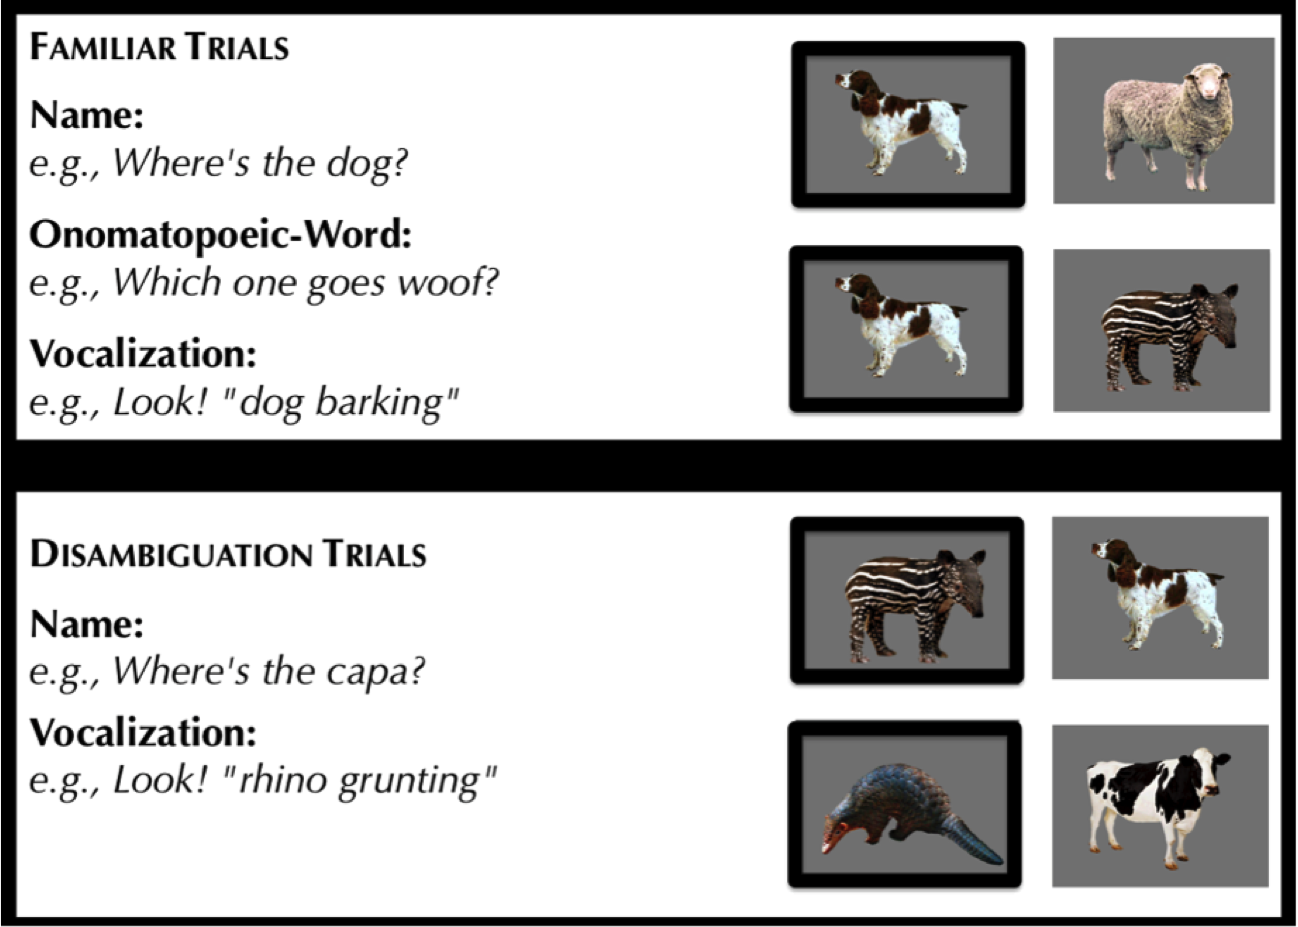
\includegraphics[width=0.95\linewidth]{anime_manuscript_files/figure-latex/stimuli-e1-1} \caption{Trial types in Experiments 1 and 2 organized by type of cue: Familiar vs. Novel. The target animal for each trial type is on the left.}\label{fig:stimuli-e1}
\end{figure}

\subsubsection{Visual stimuli}\label{visual-stimuli}

The visual stimuli included pictures of four Familiar animals (horse,
dog, cow, sheep) and two Novel animals (pangolin, tapir). According to
parental report, the familiar animals were known by all children.
Parents also reported that the novel animals were completely unfamiliar
to the children. Each animal picture was centered on a grey background
in a 640 x 480 pixel space

\subsubsection{Auditory stimuli}\label{auditory-stimuli}

The auditory stimuli consisted of sounds that were either Familiar or
Novel to 32-month-olds. Figure 1 serves as a guide to the different
sound types. The Familiar sounds were used in Familiar Trials, and
consisted of one of three different sounds: names (horse, dog, cow and
sheep), onomatopoeic words (neigh, woof-woof, moo and baa), and
vocalizations (horse neighing, dog barking, cow mooing and sheep
baaing). The Novel sounds were used in Disambiguation Trials, and
consisted of one of two types of sounds: names (capa, nadu) and
vocalizations (rhino grunting, gorilla snorting).

Trials in which the auditory cue was a familiar or novel animal name
(e.g., Where's the dog?) or a familiar or novel lexical sound (Which one
goes woof-woof?) began with a brief carrier frame. The duration of the
target cue was 810 ms for lexical sounds and 750 ms for animal names.
The intensity of the phrases was normalized using Praat speech analysis
software (Boersma, 2002).

Trials with familiar or novel animal vocalizations began with a single
word, used to draw children's attention (e.g., Look! \enquote{dog
barking}). Familiar animal vocalizations were selected based on
prototypicality. After selecting at least three vocalizations for each
familiar animal, the authors voted on the one that we thought would be
most easily recognized by children. Choosing the novel animal
vocalizations was more challenging. A group of research assistants
selected from different websites several vocalizations that they judged
as unfamiliar. From these vocalizations, we selected two (i.e., rhino
grunting and gorilla snorting) that we judged were equally likely to be
produced by the 6 familiar and 2 novel animals based on the their size
and vocal tract characteristics. These vocalizations were also maximally
distinct from each other and from the familiar animal vocalizations and
expected to be unfamiliar to children. We counterbalanced the
vocalizations that were paired with the two novel animals, in order to
control for the possibility that children judged one of the two novel
animals as more likely to produce one of the novel vocalization. All
children were reported by parents to have had no exposure to the novel
animal's natural vocalizations. The duration of the target animal
vocalizations was 2000 ms. More details about trial types and conditions
in Figure 1 will be given in the Procedure section.

\subsubsection{Familiarization books}\label{familiarization-books}

There were two main reasons for us to want to make sure that children
knew the familiar onomatopoeic words and animal vocalizations before we
administered our experiment. First, we wanted to make sure that any
differences we observed in children's performance within Familiar-Animal
Trials was due to processing speed and could not be explained by the
fact that children were not familiar with one of the sound types. The
looking-while-listening procedure has been shown to capture differences
in processing efficiency even when words are considered \enquote{known}
by offline reaching tasks or parental report (Fernald et al., 2008).
Second, we wanted to make sure that children knew the pairings between
familiar vocalizations and animals, a potential prerequisite for success
on Disambiguation trials. Since we were working with children from
mid/high-SES families growing up in an urban environment, we were
particularly concerned that they would not be familiar with many animal
vocalizations or onomatopoeic words. To ensure that all children had at
least some experience with the familiar animals and familiar auditory
cues used in our study, we gave two children's books to parents, both
titled Sounds on the Farm, a week before their visit. Parents were
instructed to share each book with their child for 5 to 10 min on at
least three days prior to the experiment. The first book consisted of
colorful pictures of each familiar animal and text designed to prompt
parents to produce each animal's lexical sound (e.g., Wow, look at all
those cows! This cow says moo, moo!). To give children exposure to the
natural animal vocalizations, we used a Hear and There book, which
contained buttons that children could press to hear the actual noise
that each animal produces.

\subsubsection{Procedure}\label{procedure}

Since we were interested in detecting differences in processing between
sounds that we expected to be familiar to children, we choose to access
speed and accuracy in identifying the correct target picture with the
looking-while-listening (LWL) procedure (see Fernald, et al, 2008).
Previous studies have shown that even when objects are reported by
parents as familiar to their children, or when children are at ceiling
in offline reaching tasks, these real-time processing measures can
capture meaningful differences in processing. These differences
correlate to properties of the sound stimuli (e.g., word-frequency) and
different aspects of the child's experience (e.g., their age,
socioeconomic status, amount of parental talk). Looking-time measures
have also been used in Disambiguation tasks with children from different
ages, capturing differences in accuracy that relate to children's age
and vocabulary size (Bion et al., 2013).

On each trial, a pair of pictures was presented on the screen for
approximately 4 s, with the auditory stimuli starting after 2 s,
followed by 1 s of silence. As seen in Figure 1, we have two main trials
types, Familiar Trials and Disambiguation trials, paralleling our
original two research questions on children's processing of familiar and
novel auditory cues.

Within the Familiar Trials, we have three different sub-trials: name,
onomatopoeic word, and vocalization. On 8 Name trials, each familiar
animal served as the target twice and was paired once with another
familiar animal and once with a novel animal. On 8 Onomatopoeic-word
trials, each familiar animal served as the target twice. On 16
Vocalization trials, each familiar animal served as the target four
times, paired twice with another familiar animal and twice with a novel
animal. These three familiar sound types should allow us to answer our
first research question, asking whether names, onomatopoeic words, or
animal vocalizations, are equally effective as acoustic cues in guiding
children's attention to animals in a visual scene.

Within the Disambiguation Trials, we have two different sub-trials:
name, and vocalizations. On 6 Name trials, each novel animal was labeled
three times with a novel animal name (i.e., capa, nadu), always paired
with a familiar animal. On 8 Vocalization trials, each novel animal
vocalization served as the target four times and was paired with each
familiar animal once. These two sound types should allow us to answer
our second research question, asking whether two-year-olds make similar
inferences when mapping a novel name and a novel animal vocalization to
an unfamiliar animal.

These different trial types were administered in two different visits.
The Familiar and Disambiguation Trials with animal names and
onomatopoeic words were administered during children's first visit. The
Familiar and Disambiguation Trials with the animal vocalizations were
administered during their second visit. We administered the animal
vocalizations on the second visit to allow children to become familiar
with the procedure and to give parents additional time to use the
familiarization books with the vocalizations with their children. During
each visit, five Filler trials were interspersed throughout to add
variety and maintain children's attention. Pairings of the novel animal
and name, and side of presentation of target animals, were
counterbalanced across participants. Caregivers wore darkened sunglasses
so that they could not see the pictures and influence infants' looking
throughout the 5-min procedure.

\subsubsection{Measures of processing
efficiency}\label{measures-of-processing-efficiency}

Participants' eye movements were video-recorded and coded with a
precision of 33 ms by observers who were blind to trial type. Inter- and
intra-observer reliability checks were conducted for all coders. For
25\% of the subjects, two measures of inter-observer reliability were
assessed. The first was the proportion of frames (33-ms units) on each
trial on which two coders agreed. In this case, agreement was 98\%.
However, because this analysis included many frames on which the child
was maintaining fixation on one picture, we also calculated a more
stringent test of reliability. This second measure focused only on
shifts in gaze, ignoring steady-state fixations in each trial on which
agreement was inevitably high. By this more conservative measure, coders
agreed within one frame on 94\% of all shifts.

\textbf{Accuracy:} On those trials in which the infant was fixating a
picture at the onset of the speech stimulus, accuracy was computed by
dividing the time looking to the target object by the time looking to
both target and distracter, from 300 to 2500 ms from the onset of the
target word. Accuracy before 300 ms was not included because shifts to
the target occurring in this window had presumably been initiated before
the onset of the noun. This analyses window was chosen because of the
longer duration of the animal vocalizations (2 s.) and because of the
introduction of novel auditory cues. A single analyses window was used
for all trial types for consistency. Mean accuracy was then computed for
each participant on each trial type.

\textbf{Reaction time:} We calculated reaction time (RT) on those trials
on which participants were looking at the distractor animal at the
beginning of the sound. RT on each trial was the latency of the first
shift to the correct animal within a 300- to 1,800-ms window from sound
onset, as typically done in studies using this procedure (Fernald et
al., 2008).

\subsection{Results and discussion}\label{results-and-discussion}

\subsubsection{Familiar Trials: Using familiar animal names, onomatopeic
sounds, and animal vocalization to identify familiar
animals:}\label{familiar-trials-using-familiar-animal-names-onomatopeic-sounds-and-animal-vocalization-to-identify-familiar-animals}

Our first question is whether a familiar animal name, onomatopoeic word,
and animal vocalization are equally effective in guiding children's
attention to an animal in the visual scene. Figure 2A shows children's
looking behavior over time on the LWL procedure (Fernald et al., 1998).
In order to capture children's speed of processing, we show children's
responses on trials in which they start looking at the wrong animal.
From sound onset onward, we show the mean proportion of trials in which
children were looking at the correct picture, every 33ms, with different
lines representing children's responses on Name trials (black),
Onomatopoeic-word trials (light grey), and Vocalization trials (dark
grey). The y-axis shows the mean proportion of trials on which children
were looking at the correct animal. The x-axis represents time from
sound onset in milliseconds. Around 750ms from sound onset there is
already a substantial difference in the mean proportion of trials in
which children are looking at the correct animal depending on whether
they heard an animal name or an animal vocalization. Children are
looking at the correct animal in a greater proportion of trials when
they hear a familiar animal name, as compared to when they hear an
animal vocalization, with performance on trials with onomatopoeic words
falling between the two.

To quantify these differences, we fit Bayesian mixed-effects regression
models using the \texttt{rstanarm} (Gabry \& Goodrich, 2016) package in
R (3.4.1, R Core Team, 2017)\footnote{We, furthermore, used the
  R-packages \emph{here} (0.1, Müller, 2017), \emph{knitr} (1.17, Xie,
  2015), \emph{papaja} (0.1.0.9492, Aust \& Barth, 2017), and
  \emph{tidyverse} (1.2.1, Wickham, 2017).}. The mixed-effects approach
allowed us to model the nested structure in our data by including random
intercepts for each participant and item and a random slope for each
item. We used Bayesian methods in order to quantify support in favor of
null hypotheses of interest -- in this case, the absence of a difference
in real-time processing across the different familiar cue types. To
communicate the uncertainty in our estimates, we report the 95\% Highest
Density Interval (HDI) around the point estimates of the group means and
the difference in means. The HDI provides a range of plausible parameter
values given the data and the model. All analysis code can be found in
the online repository for this project:
\url{https://github.com/kemacdonald/anime}.

We computed reaction time (RT) as the mean time it took them to shift to
the correct picture on trials in which they were looking at the wrong
picture at sound onset for the three cue types. To make RTs more
suitable for modeling on a linear scale, we analyzed responses in log
space using a logistic transformation, with the final model was
specified as: \(log(RT) \sim cue\_type + (1 + sub\_id \mid item)\).

Figure 2 shows the data distribution for each participant's RT, the
estimates of condition means, and the full posterior distribution of
condition differences across the different cue types. Children were
faster to identify the target animal while hearing its name
(\(M_{name}\) = 876.35 ms), as compared to its onomatopeic animal sound
(\(M_{onomatopeia}\) = 649.70 ms), and its vocalization
(\(M_{vocalization}\) = 720.38 ms). The difference between RTs for the
name and onomatopeic animal sounds was -70.67 ms with a HDI from -212.86
ms to 68.88 ms. While the null value of zero difference falls within the
95\% HDI, 83.50\% of the credible values fall below the null, providing
some evidence for faster processing of animal names. The average
difference in children's RT between the name and vocalization trials was
-226.65 ms with a HDI from -361.37 ms to -85.23 ms and 99.95\% of the
credible values falling below zero, providing strong evidence that
children processed names more efficiently compared to vocalizations.
Finally, the average difference in children's RT between the onomatopeic
sounds and vocalization trials was -155.98 ms with a HDI from -301.18 ms
to -5.77 ms and 97.95\% of the credible values falling below zero.

Together, the RT modeling results provide strong evidence that children
processed animal names around 227 ms faster than animal vocalizations,
with almost all of the estimates of the plausible RT differences falling
below the null value of zero. There was slightly weaker evidence that
children processed animal names more efficiently compared to onomatopeic
animal sounds but strong evidence of faster processing of onomatopeic
animal sounds compared to animal vocalizations. In sum, there was
evidence of a graded effect of cue type on RTs with names being faster
than onomatopeic animal sounds, which were faster than animal
vocalizations.

\begin{figure}[H]
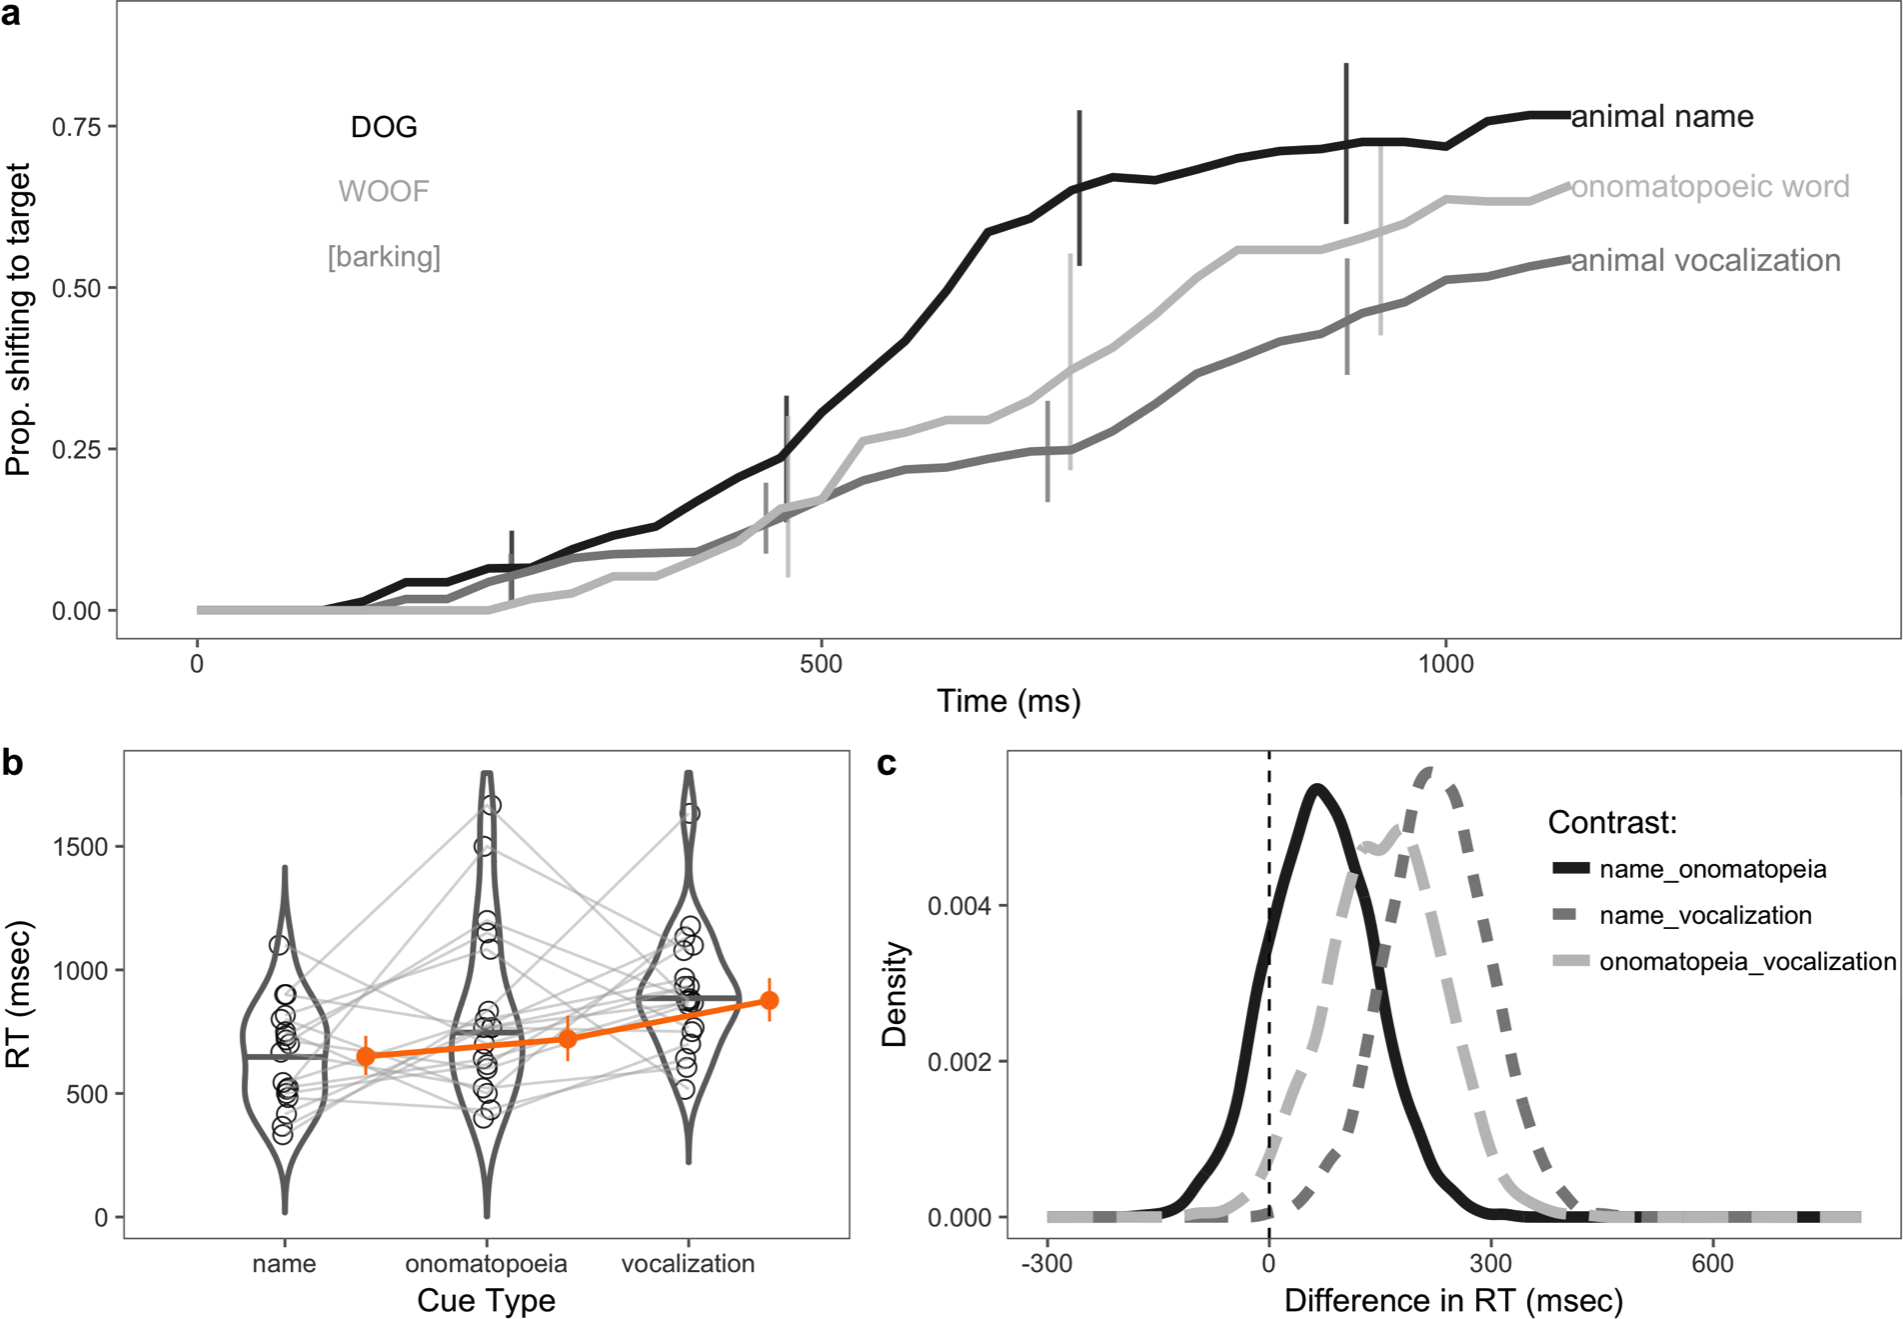
\includegraphics[width=0.95\linewidth]{anime_manuscript_files/figure-latex/oc-plot-e1-1} \caption{Reaction Time (RT) results for Experiment 1. Panel A shows the time course of children’s looking to the target animal after hearing a familiar animal name (black), onomatopoeic word (light grey), or animal vocalization (dark grey). The x-axis shows time in milliseconds from sound onset. The y-axis shows the mean proportion of trials in which children are looking to the target animal. Panel B shows the distribution of RT data and the estimate of group means for RT (orange points). Each grey point represents and light grey line shows a single child's performance acrossthe different cue types. The orange points represent the most likely estimate of the group means with the error bars showing the 95\% HDI. Panel C shows the posterior distribution over RT differences across conditions. Color and linetype represent the contrast and the vertical dashed line represents the null value of zero difference.}\label{fig:oc-plot-e1}
\end{figure}

Children's reaction times showed a difference in speed of processing for
names, onomatopoeic words, and vocalization. Next, we estimated
children's attention to the target image over the course of the trial to
ask whether the three trial types were equally effective cues to guide
their attention to a familiar animal. We computed accuracy over a window
from 300 to 2500 ms after the onset of the cue. The upper left panel of
Figure 3A shows children's proportion looking to the target for each
trial type. Each point represents a single participant's Accuracy, the
grey line shows the full distribution of the data, and the horizontal
line shows the median value. The orange points represent the most likely
estimate for the mean proportion looking with the error bars showing the
95\% HDI. Visual inspection of the plot suggests two things: (1)
children reliably looked to the correct animal after hearing each of the
three familiar cues and (2) children's overall looking behavior was
strikingly similar across conditions.

Next, we quantified the strength of evidence for the absence of any
condition differences and for the difference from random responding. We
estimated the mean proportion looking for each trial type using a
Bayesian linear mixed-effects model with the same specifications as the
RT model described above. We transformed the proprotion looking scores
using the empirical logit, with the final model as:
\(logit(accuracy) \sim cue\_type + (1 + sub\_id \mid item)\). The orange
points in Figure 3A show mean Accuracy for each familiar cue type
(\(M_{name}\) = 0.66, \(M_{onomatopeia}\) = 0.68, and
(\(M_{vocalization}\) = 0.67). Children's looking to the target image
was reliably different from a model of random looking behavior across
all conditions, with the null value of 0.5 falling well outside of the
range of plausible values (see the difference between the horizontal
dashed line and error bars in Figure 3A).

Moreover, the three cues types were equally effective in guiding
children's attention to the target animal over the course of the trial
as shown by the high overlap in the posterior distributions of Accuracy
and that the null value of zero difference fell within the HDI for all
group comparisons (name vs.~onomatopeia: \(\beta_{diff}\) = 0.03, 95\%
HDI from -0.07 to 0.11; name vs.~vocalization: \(\beta_{diff}\) = 0.01,
95\% HDI from -0.05 to 0.08; onomatopeia vs.~vocalization:
\(\beta_{diff}\) = -0.01, 95\% HDI from -0.09 to 0.07). These results
provide strong evidence that the animal vocalizations were equally
effective at directing overall looking behavior to identify familiar
animals as their names or onomatopeic sounds if children have enough
time to process the cue.

\subsubsection{Disambiguation Trials: Using novel animal names and
animal vocalization to disambiguate novel
animals}\label{disambiguation-trials-using-novel-animal-names-and-animal-vocalization-to-disambiguate-novel-animals}

Our next question is whether children would orient to a novel animal
after hearing a novel animal name or vocalization, thus showing evidence
of one-to-one biases for the vocalizations that animals produce. We
focus on children's accuracy, comparing their proportion of looking to
the novel animal against chance performance and across cue types. The
orange points in Figure 3A show Accuracy group means for each novel cue
type (\(M_{name}\) = 0.69 ms, \(M_{vocalization}\) = 0.70). Children's
looking to the target image was reliably different from a model of
random looking behavior across both cue types, with the null value of
0.5 falling well outside of the range of plausible values.

Moreover, the novel animal name and animal vocalizations were equally
effective in guiding children's attention to the target animal over the
course of the trial (name vs.~onomatopeia: \(\beta_{diff}\) = 0.01, 95\%
HDI from -0.05 to 0.08). This result provides strong evidence that the
animal vocalizations were equally effective at directing overall looking
behavior to identify familiar animals as their names or onomatopeic
sounds if children have enough time to process the cue.

\begin{figure}[tb]
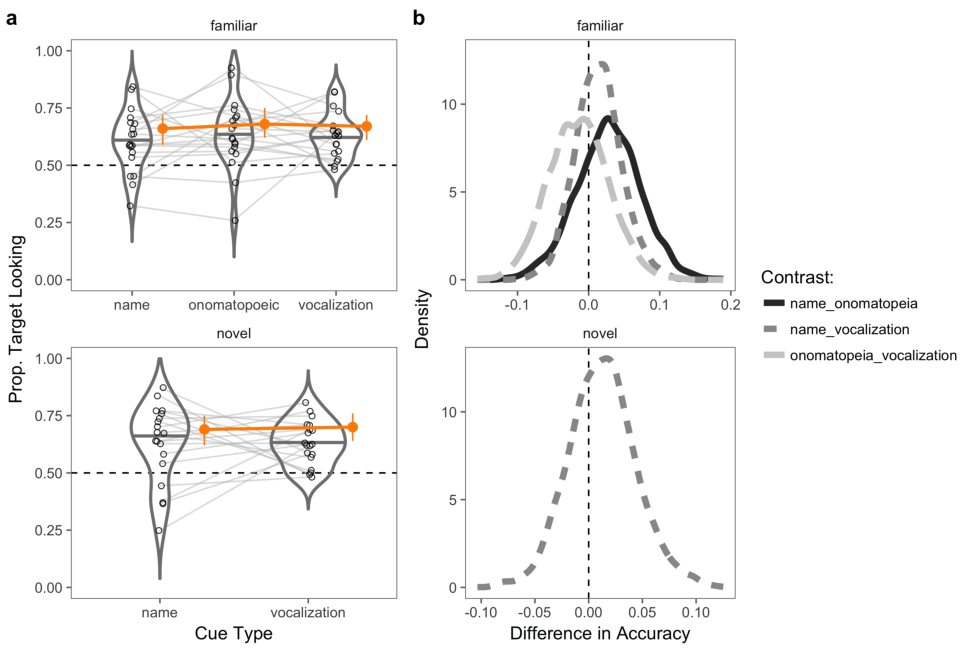
\includegraphics[width=0.95\linewidth]{anime_manuscript_files/figure-latex/acc-plot-e1-1} \caption{Accuracy results for Experiment 1 for familiar (upper panels) and novel (lower panels) trials. Panel A shows the data distribution and model estimates for Accuracy of children's looking behavior. Panel B shows the full posterior distribution over model estimates of differences in accuracy across conditions. The vertical dashed line represents the null model of zero difference in Accuracy. All other plotting conventions are the same as in Figure 2.}\label{fig:acc-plot-e1}
\end{figure}

Therefore, children seem to have one-to-one biases for the vocalizations
that animals produce already at 30 months of age, the earliest age at
which the disambiguation effect has been observed in a domain other than
word learning. There were no significant differences between children's
reaction time for novel animal names or vocalizations.

\section{Experiment 2}\label{experiment-2}

An issue that has received much attention in recent years concerns the
relation between children's referent selection and retention abilities.
While earlier studies tended to conflate disambiguation strategies and
children's word learning, more recent studies suggest that these two
abilities should not be conflated (Bion, Borovsky, \& Fernald, 2013;
Horst \& Samuelson, 2008)

Horst and Samuelson (2008) examined both referent selection and
retention in four experiments with 2-year-olds. When children were shown
a novel object among familiar objects, they selected the novel object
when hearing a novel label, as found in previous studies. But
surprisingly, on retention trials 5 min later, these children showed no
evidence of remembering the names of the novel objects they had
previously identified. Using a looking-time task, Bion et al. (2013)
replicated these findings in a study with 18-, 24-, and 30-month-old
infants using looking time measures of performance.

Experiment 2 asks whether children can retain the link created through
disambiguation between a novel animal and a novel animal vocalization.
In addition, we aim at replicating the findings from Experiment 1,
showing that children can identify familiar animals based on the
vocalizations they produce, and use novel vocalizations to disambiguate
novel animals. Our prediction is that children will succeed in
disambiguation trials, but will show marginal or no retention on
subsequent disambiguation trials, paralleling the findings of earlier
studies with linguistic stimuli.

\subsection{Method}\label{method-1}

\subsubsection{Participants}\label{participants-1}

Participants were 23 31-month-old children (M = 31.10 months; range = 30
- 32), 12 girls. All children were typically developing and from
families where English was the dominant language.

\subsubsection{Visual stimuli}\label{visual-stimuli-1}

The visual stimuli were the same as in Experiment 1, except for the
novel animals (aardvark and capybara), which replaced the novel animals
(pangolin and tapir) used in Experiment 1 (see animals in Figure 4). We
decided to change the novel animals in order to confirm that our results
were not restricted to the particular stimuli set in Experiment 1. All
children were reported by parents to have had no exposure to the novel
animals.

\subsubsection{Auditory stimuli}\label{auditory-stimuli-1}

The auditory stimuli consisted of the same familiar and novel animal
vocalizations as in Experiment 1.

\begin{figure}[tb]
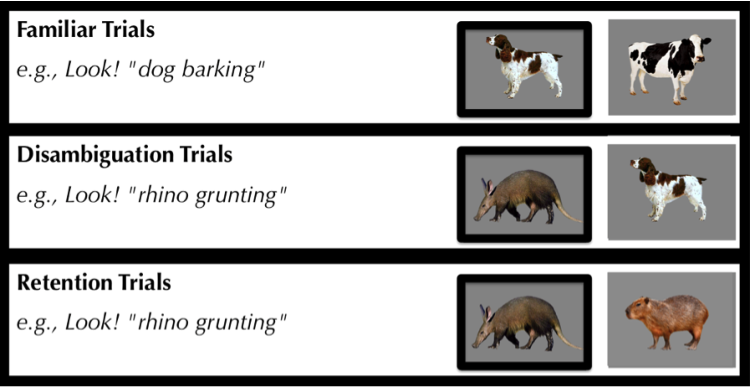
\includegraphics[width=0.95\linewidth]{anime_manuscript_files/figure-latex/stimuli-e2-1} \caption{Trial types in Experiments 4 organized by type of trial. Children hear familiar and novel vocalizations. The target animal for each trial type is on the left.}\label{fig:stimuli-e2}
\end{figure}

\subsubsection{Familiarization books}\label{familiarization-books-1}

As in Experiment 1, we sent home a children's book to ensure that all
participants had at least some exposure to the familiar animals and
auditory cues. Since, in Experiment 2, we were interested in the natural
animal vocalizations and not the names/lexical sounds, only the Hear and
ThereTM Sounds on the Farm book was used. Instructions given to the
parents were the same as in Experiment 1, and the book was sent home a
week before the visit.

\subsubsection{Procedure}\label{procedure-1}

Experiment 2 consisted of one visit. Each child saw 30 trials,
consisting of three trial types (Figure 4). The 16 Familiar trials and 8
Disambiguation trials were identical in structure to the Vocalization
trials Experiment 1. In addition, on 6 Retention trials, the two novel
animals were presented side by side, with each serving as the target
three times. The same coding and speed/accuracy measures were used as in
Experiment 1.

\subsection{Results and discussion}\label{results-and-discussion-1}

\subsubsection{Retention of the link between a novel animal and a novel
vocalization:}\label{retention-of-the-link-between-a-novel-animal-and-a-novel-vocalization}

Figure 5A shows children's proportion looking to the target animal after
hearing a familiar or a novel animal vocalization over the same analysis
window used in Experiment 1 (300 to 2500 ms after the onset of the
vocalization). Visual inspection of the figure suggest that children
successfully oriented to the target image after hearing both familiar
and novel animal vocalizations. The orange points show mean proportion
target looking for familiar (\(M_{familiar}\) = 0.66, disambiguation
(\(M_{disambiguation}\) = 0.64, and retention trials (\(M_{retention}\)
= 0.50).

Children's looking to the target image was reliably different from
random looking behavior for both familiar and disambiguation trials,
with the null value of 0.50 falling well outside of the range of
plausible values. Moreover, the novel animal vocalizations and the
familiar animal vocalizations were equally effective in guiding
children's attention to the target animal over the course of the trial
(familiar vs.~disambiguation: \(\beta_{diff}\) = 0.02, 95\% HDI from
-0.08 to 0.11).

In contrast to children's success on familiar trials and disambiguation
trials, they did not show evidence of retaining the link between the
novel animal and the novel animal vocalization, with the null value of
\(0.5\) proportion looking falling well within the range of plausible
estimates. Moreover, there was strong evidence that children were less
accurate on retention trials compared to both disambiguation trials
(\(\beta_{diff}\) = 0.14, 95\% HDI from 0.03 to 0.25) and familiar
trials (\(\beta_{diff}\) = 0.16, 95\% HDI from 0.05 to 0.27).

\begin{figure}[tb]
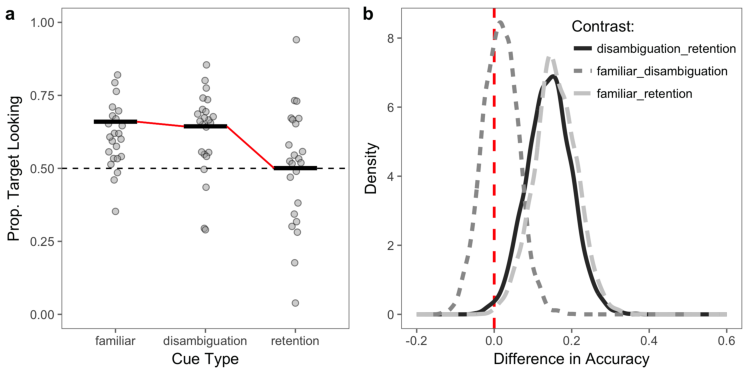
\includegraphics[width=0.95\linewidth]{anime_manuscript_files/figure-latex/acc-plot-e2-1} \caption{Accuracy of responses to familiar and novel animal vocalizations in Experiment 2. Panel A shows the data distribution alongside the model estimates of mean Accuracy across the different trial types. Panel B shows the full posterior distribution over model estimates of differences in accuracy across trial types. The vertical dashed line represents the null model of zero difference. All other plotting conventions are the same as in Figures 1 and 2.}\label{fig:acc-plot-e2}
\end{figure}

Three findings emerged from the accuracy analysis: First, children
oriented to a familiar animal after hearing a familiar animal
vocalization. Second, children oriented to a novel animal after hearing
a novel animal vocalization. These two results are an internal
replication of the key findings from Experiment 1 in a new sample. In
addition, we found that children did not show evidence of retaining the
link between a novel animal vocalization and a novel animal. These
results and their implications will be discussed in more details in the
following section.

\section{General Discussion}\label{general-discussion}

Three main findings emerged from this work. The first finding was that
30-month-olds responded fastest to a familiar animal name and slowest to
a familiar animal vocalization, with onomatopoeic sounds falling
somewhere in between. Yet, children could identify the familiar animals
after hearing any of on these three sound types. The second finding was
that children showed disambiguation biases for the types of
vocalizations that animals produce, similar to their biases in word
learning. The third finding was that these biases do not necessarily
lead to learning, as children were not successful in retaining the link
between novel animals and their vocalizations. This lack retention
parallels the findings of recent word-learning studies (see McMurray,
Horst, Toscano, and Samuelson (2009)) and emphasizes the theoretical
importance of disentangling processes of disambiguating reference, an
in-the-moment phenomenon, and word learning, which occurs over a longer
timescale.

In our study, we found a processing speed advantage for words over other
meaningful sounds. Some theories of language development argue that
words are a unique stimuli because they refer to objects in the world
(Waxman \& Gelman, 2009), while other theories argue that words are
special because they activate conceptual information more quickly,
accurately, and in a more categorical way than nonverbal sounds. It is
also possible that words and nonverbal sounds might be processed by
different brain regions, with words being accessed more rapidly. A
second explanation for the advantage for words might be differences in
sheer frequency in the input. At least in our sample, it is safe to
assume that children have heard the word cow many more times than they
have heard an actual cow mooing. Frequency effects have been robustly
demonstrated in the processing of words, with adults being faster to
recognize words that they hear more frequently (Dahan, Magnuson, \&
Tanenhaus, 2001). A final explanation is that words are very effective
at presenting a lot of information in a short period of time. When
children see a simple visual world consisting of a dog and a sheep, the
first phoneme of the target word is already sufficient to determine the
animal that is likely to be talked about next.

Much less is known about children's and adults' processing of
onomatopoeic sounds. Hashimoto et al. (2006) compared brain responses to
nouns, animal sounds, and onomatopoetic sounds, and found that
onomatopoeic sounds were processed by extensive brain regions involved
in the processing of both verbal and nonverbal sounds. Alycia Cummings
et al. (2009) argues that onomatopoeic sounds might provide young
children with information about intermodal associations, bridging their
understanding of non-arbitrary environmental sounds and arbitrary
word-object associations. Fernald and Morikawa (1993) reported that 52\%
of Japanese mothers used onomatopoeic sounds to label target objects,
while only 1 in 30 American mothers did so. While our results do not
speak direclty to these theoretical issues, they do suggest that
onomatopoeic sounds function like words in that they are capable of
activating conceptual representations that drive children's visual
attention to seek the physical referent of the sound. However, there was
some evidence that children processed onomatopeic sounds less
efficiently compared to words in our task.

Our second finding was that children looked at a novel animal when
hearing a novel animal vocalization, with accuracy comparable to their
disambiguation of novel animal names. Bloom (2002) discusses different
theories explaining children's disambiguation biases: These biases could
be a specifically lexical phenomenon that applies only to words (lexical
account), a product of children's theory of mind restricted to
communicative situations (pragmatic account), or a special case of a
general principle of learning that exaggerates regularities across
domains (domain-general account). This study represents a strong test of
these different accounts since they make different predictions for
children's looking behavior in response to the sounds that animals make,
a non-linguistic and non-communicative stimulus.

Previous studies contrasted lexical-specific and pragmatic accounts,
with little attention to domain-general explanations. Diesendruk and
Markson found that children expect speakers to use consistent facts to
refer to objects, and they select a novel object when hearing a novel
fact (Diesendruck \& Markson, 2001). Yet, recent studies suggest that
different strategies might be used to make inferences about speakers'
communicative intent and the meaning of a novel word. Autistic children
who are known to have pragmatic deficits show disambiguation biases and
select a novel word when hearing a novel object (Preissler \& Carey,
2005). Disambiguation biases for words are correlated with vocabulary,
and disambiguation biases for facts are correlated with social-pragmatic
skills (Marchena et al., 2011). As these authors acknowledge, these
findings suggest that disambiguation biases for words might not be
motivated uniquely by pragmatic inferences, but they do not rule out
domain-general accounts.

Few studies looked at disambiguation biases in non-linguistic domains.
Three-year-olds expect faces to map to individual voices (Moher,
Feigenson, \& Halberda, 2010), showing that one-to-one biases might
extend to other communicative domains. In contrast, studies with adults
found an advantage for words over non-linguistic stimuli in a task that
could benefit from disambiguation biases (Yoshida, Rhemtulla, \&
Vouloumanos, 2012). The findings with adults do not rule out a
domain-general account, since participants had no reason to expect that
the mapping between random non-linguistic sounds and objects should be
mutually exclusive. As pointed out by the authors, perhaps similar
strategies might be applied to non-linguistic sounds if they were
meaningfully related to the object.

This study is the first to demonstrate that young children show
disambiguation biases in a non-linguistic and non-communicative domain.
This is also the youngest age at which disambiguation biases were shown
in a domain other than word learning. These findings seem to favor
domain-general accounts that see disambiguation biases as the natural
consequence of a system that attempts to find regularities in complex
learning tasks that involve consistent mappings. Previous connectionist
and Bayesian models of word learning showed that disambiguation biases
emerge as children are exposed to consistent mappings between words and
objects, without the need of built-in constraints on the meaning of
words (M. C. Frank et al., 2009; McMurray et al., 2012; Regier, 2003).
In principle, these same biases would emerge if these models attempted
to map animal vocalizations to animals and consistent co-occurrences
were present in the environment.

The question that remains is whether the finding from our studies and
from previous studies could be explained by a single disambiguation
mechanism. We showed that children can disambiguate stimuli other than
words and facts, suggesting at least the existence of a domain general
mechanism that leads to disambiguation. A preference for parsimony
provides some week evidence in favor of a single mechanism. But as
pointed out by recent computational work, it is possible that different
mechanisms jointly contribute to disambiguation behavior, explaining
findings across different populations and contexts (Lewis \& Frank,
2013). It is possible therefore that the same behavior - selecting a
novel object when hearing a novel auditory stimulus - might result from
different computational mechanisms or motivations depending on the task
at hand, children's age, or the particular stimuli set and assumptions
about the people involved in the interaction. That is, children could
use a domain general mechanism to learn about novel animal
vocalizations, and they could use a lexical and pragmatic constraint to
learn about novel words.

Our third finding was that one-to-one biases for animal vocalizations do
not necessarily lead to retention of the link between a novel animal and
a novel vocalization. Importantly, this finding supports the prediction
of recent cross-situational models of early word learning (McMurray et
al., 2012). McMurray and colleagues propose that referent-selection
requires that children give their best guess about a new word's meaning
in a specific ambiguous situation, but that learning operates over a
much longer timescale. Although disambiguation can be viewed as the
product of learning that has occurred up to that point, for younger
children it does not necessarily result in learning. These claims are
also supported by evidence from studies on early word learning using
online and offline measures of retention (Bion et al., 2013).

These results also add to a recent body of work that encourages us to
think differently about disambiguation biases. This work has emphasized
the role of experience in the emergence of disambiguation biases,
showing that the tendency to select a novel object when hearing a novel
word is not robustly present across populations. For example, bilingual
children, children from lower socioeconomic status, children who receive
less language input, and children with less structured vocabularies or
smaller vocabulary sizes, take longer to show evidence of disambiguation
biases (Bion et al., 2013; Yurovsky, Bion, Smith, \& Fernald, 2012).
Other studies have problematized the relation between disambiguation
biases and word learning, showing that success in referent selection
does not necessarily mean that the link between the novel word and novel
object will be retained (Bion et al., 2013; Horst, McMurray, \&
Samuelson, 2006; McMurray et al., 2012). And the current study adds to
recent studies taking a fresh look at an old question: the scope of
disambiguation biases (Suanda \& Namy, 2012, 2013). Taken together,
these recent studies challenge some widespread assumptions about the
emergence, importance, and scope of a behavior often characterized as
innate and universal.

Children's learning about objects in their environment involves more
than learning their names. Before object names are learned, sounds and
actions might form the basis on which objects are conceptualized. For
example, children might see barking as a defining feature of dogs, and
may say bow-wow in response to the picture of a dog, even before they
learn the animal name (Nelson, 1974). Learning the meaning of an object
therefore requires learning several cross-modal associations, including
learning the object's texture, smell, as well as its sounds and names.
Children do not have explicit constraints that freshly baked cookies
should have only one smell. Yet, they might recognize and get excited
about the familiar smell coming from the kitchen, and might assume their
mothers are baking something new when smelling something unfamiliar.

Children use different types of knowledge in order to make sense of a
constantly changing world. They might identify animal vocalizations
based on the shape of the vocal tract of the animal, its location and
size, and their previous knowledge about animal vocalizations.
Importantly, these cues normally converge in helping children identify
an animal in the environment. The same is true for their identification
of referents for words. Children can identify the referent for a word
based on semantics (J. C. Goodman, McDonough, \& Brown, 1998),
cross-situational statistics (Smith \& Yu, 2008), syntax (R. W. Brown,
1957), and pragmatic and social cues (Baldwin, 1993), and -- why not -
disambiguation biases {[}markman1991whole{]}. As children grow older,
these different sources of information provide converging evidence that
a novel word should refer to a novel object. Children can rely on their
knowledge about the world, speakers, and on their previous experiences
with words in order to figure out what speakers are talking about -- a
task we continue to do throughout our lives when learning knew words and
interpreting complex sentences.

\newpage

\section{References}\label{references}

\setlength{\parindent}{-0.5in} \setlength{\leftskip}{0.5in}

\hypertarget{refs}{}
\hypertarget{ref-R-papaja}{}
Aust, F., \& Barth, M. (2017). \emph{papaja: Create APA manuscripts with
R Markdown}. Retrieved from \url{https://github.com/crsh/papaja}

\hypertarget{ref-baldwin1993infants}{}
Baldwin, D. A. (1993). Infants' ability to consult the speaker for clues
to word reference. \emph{Journal of Child Language}, \emph{20}(02),
395--418.

\hypertarget{ref-bates1989functionalism}{}
Bates, E., MacWhinney, B., \& others. (1989). Functionalism and the
competition model. \emph{The Crosslinguistic Study of Sentence
Processing}, \emph{3}, 73--112.

\hypertarget{ref-bion2013fast}{}
Bion, R. A., Borovsky, A., \& Fernald, A. (2013). Fast mapping, slow
learning: Disambiguation of novel word--object mappings in relation to
vocabulary learning at 18, 24, and 30months. \emph{Cognition},
\emph{126}(1), 39--53.

\hypertarget{ref-bloom2002children}{}
Bloom, P. (2002). \emph{How children learn the meaning of words}. The
MIT Press.

\hypertarget{ref-brown1957linguistic}{}
Brown, R. W. (1957). Linguistic determinism and the part of speech.
\emph{The Journal of Abnormal and Social Psychology}, \emph{55}(1), 1.

\hypertarget{ref-chen2011crossmodal}{}
Chen, Y.-C., \& Spence, C. (2011). Crossmodal semantic priming by
naturalistic sounds and spoken words enhances visual sensitivity.
\emph{Journal of Experimental Psychology: Human Perception and
Performance}, \emph{37}(5), 1554.

\hypertarget{ref-clark1990pragmatics}{}
Clark, E. V. (1990). On the pragmatics of contrast. \emph{Journal of
Child Language}, \emph{17}(2), 417--431.

\hypertarget{ref-cummings2010verbal}{}
Cummings, A., \& Ceponiene, R. (2010). Verbal and nonverbal semantic
processing in children with developmental language impairment.
\emph{Neuropsychologia}, \emph{48}(1), 77--85.

\hypertarget{ref-cummings2006auditory}{}
Cummings, A., Ceponiene, R., Koyama, A., Saygin, A., Townsend, J., \&
Dick, F. (2006). Auditory semantic networks for words and natural
sounds. \emph{Brain Research}, \emph{1115}(1), 92--107.

\hypertarget{ref-cummings2009infants}{}
Cummings, A., Saygin, A. P., Bates, E., \& Dick, F. (2009). Infants'
recognition of meaningful verbal and nonverbal sounds. \emph{Language
Learning and Development}, \emph{5}(3), 172--190.

\hypertarget{ref-dahan2001time}{}
Dahan, D., Magnuson, J. S., \& Tanenhaus, M. K. (2001). Time course of
frequency effects in spoken-word recognition: Evidence from eye
movements. \emph{Cognitive Psychology}, \emph{42}(4), 317--367.

\hypertarget{ref-diesendruck2001children}{}
Diesendruck, G., \& Markson, L. (2001). Children's avoidance of lexical
overlap: A pragmatic account. \emph{Developmental Psychology},
\emph{37}(5), 630--641.

\hypertarget{ref-fernald1993common}{}
Fernald, A., \& Morikawa, H. (1993). Common themes and cultural
variations in japanese and american mothers' speech to infants.
\emph{Child Development}, \emph{64}(3), 637--656.

\hypertarget{ref-fernald1998rapid}{}
Fernald, A., Pinto, J. P., Swingley, D., Weinbergy, A., \& McRoberts, G.
W. (1998). Rapid gains in speed of verbal processing by infants in the
2nd year. \emph{Psychological Science}, \emph{9}(3), 228--231.

\hypertarget{ref-fernald2008looking}{}
Fernald, A., Zangl, R., Portillo, A. L., \& Marchman, V. A. (2008).
Looking while listening: Using eye movements to monitor spoken language.
\emph{Developmental Psycholinguistics: On-Line Methods in Children's
Language Processing}, \emph{44}, 97.

\hypertarget{ref-frank2009using}{}
Frank, M. C., Goodman, N. D., \& Tenenbaum, J. B. (2009). Using
speakers' referential intentions to model early cross-situational word
learning. \emph{Psychological Science}, \emph{20}(5), 578--585.

\hypertarget{ref-fulkerson2007words}{}
Fulkerson, A. L., \& Waxman, S. R. (2007). Words (but not tones)
facilitate object categorization: Evidence from 6-and 12-month-olds.
\emph{Cognition}, \emph{105}(1), 218--228.

\hypertarget{ref-gabry2016rstanarm}{}
Gabry, J., \& Goodrich, B. (2016). Rstanarm: Bayesian applied regression
modeling via stan. r package version 2.10. 0.

\hypertarget{ref-goodman1998role}{}
Goodman, J. C., McDonough, L., \& Brown, N. B. (1998). The role of
semantic context and memory in the acquisition of novel nouns.
\emph{Child Development}, \emph{69}(5), 1330--1344.

\hypertarget{ref-hashimoto2006neural}{}
Hashimoto, T., Usui, N., Taira, M., Nose, I., Haji, T., \& Kojima, S.
(2006). The neural mechanism associated with the processing of
onomatopoeic sounds. \emph{Neuroimage}, \emph{31}(4), 1762--1770.

\hypertarget{ref-horst2008fast}{}
Horst, J. S., \& Samuelson, L. K. (2008). Fast mapping but poor
retention by 24-month-old infants. \emph{Infancy}, \emph{13}(2),
128--157.

\hypertarget{ref-horst2006online}{}
Horst, J. S., McMurray, B., \& Samuelson, L. K. (2006). Online
processing is essential for learning: Understanding fast mapping and
word learning in a dynamic connectionist architecture. In
\emph{Proceedings of the cognitive science society} (Vol. 28).

\hypertarget{ref-lewis2013integrated}{}
Lewis, M., \& Frank, M. (2013). An integrated model of concept learning
and word-concept mapping. In \emph{Proceedings of the annual meeting of
the cognitive science society} (Vol. 35).

\hypertarget{ref-lupyan2012evocative}{}
Lupyan, G., \& Thompson-Schill, S. L. (2012). The evocative power of
words: Activation of concepts by verbal and nonverbal means.
\emph{Journal of Experimental Psychology: General}, \emph{141}(1), 170.

\hypertarget{ref-de2011mutual}{}
Marchena, A. de, Eigsti, I.-M., Worek, A., Ono, K. E., \& Snedeker, J.
(2011). Mutual exclusivity in autism spectrum disorders: Testing the
pragmatic hypothesis. \emph{Cognition}, \emph{119}(1), 96--113.

\hypertarget{ref-markman1991whole}{}
Markman, E. M. (1991). The whole-object, taxonomic, and mutual
exclusivity assumptions as initial constraints on word meanings.
\emph{Perspectives on Language and Thought: Interrelations in
Development}, 72--106.

\hypertarget{ref-mccleery2010neural}{}
McCleery, J. P., Ceponiene, R., Burner, K. M., Townsend, J., Kinnear,
M., \& Schreibman, L. (2010). Neural correlates of verbal and nonverbal
semantic integration in children with autism spectrum disorders.
\emph{Journal of Child Psychology and Psychiatry}, \emph{51}(3),
277--286.

\hypertarget{ref-mcmurray2012word}{}
McMurray, B., Horst, J. S., \& Samuelson, L. K. (2012). Word learning
emerges from the interaction of online referent selection and slow
associative learning. \emph{Psychological Review}, \emph{119}(4), 831.

\hypertarget{ref-mcmurray2009integrating}{}
McMurray, B., Horst, J. S., Toscano, J. C., \& Samuelson, L. K. (2009).
Integrating connectionist learning and dynamical systems processing:
Case studies in speech and lexical development. \emph{Toward a Unified
Theory of Development: Connectionism and Dynamic Systems Theory
Re-Considered}, 218--249.

\hypertarget{ref-moher2010one}{}
Moher, M., Feigenson, L., \& Halberda, J. (2010). A one-to-one bias and
fast mapping support preschoolers' learning about faces and voices.
\emph{Cognitive Science}, \emph{34}(5), 719--751.

\hypertarget{ref-murray2006rapid}{}
Murray, M. M., Camen, C., Andino, S. L. G., Bovet, P., \& Clarke, S.
(2006). Rapid brain discrimination of sounds of objects. \emph{Journal
of Neuroscience}, \emph{26}(4), 1293--1302.

\hypertarget{ref-R-here}{}
Müller, K. (2017). \emph{Here: A simpler way to find your files}.
Retrieved from \url{https://CRAN.R-project.org/package=here}

\hypertarget{ref-namy1998words}{}
Namy, L. L., \& Waxman, S. R. (1998). Words and gestures: Infants'
interpretations of different forms of symbolic reference. \emph{Child
Development}, \emph{69}(2), 295--308.

\hypertarget{ref-nelson1974concept}{}
Nelson, K. (1974). Concept, word, and sentence: Interrelations in
acquisition and development. \emph{Psychological Review}, \emph{81}(4),
267.

\hypertarget{ref-pena2003sounds}{}
Pena, M., Maki, A., Kovac, D., Dehaene-Lambertz, G., Koizumi, H.,
Bouquet, F., \& Mehler, J. (2003). Sounds and silence: An optical
topography study of language recognition at birth. \emph{Proceedings of
the National Academy of Sciences}, \emph{100}(20), 11702--11705.

\hypertarget{ref-preissler2005role}{}
Preissler, M. A., \& Carey, S. (2005). The role of inferences about
referential intent in word learning: Evidence from autism.
\emph{Cognition}, \emph{97}(1), B13--B23.

\hypertarget{ref-R-base}{}
R Core Team. (2017). \emph{R: A language and environment for statistical
computing}. Vienna, Austria: R Foundation for Statistical Computing.
Retrieved from \url{https://www.R-project.org/}

\hypertarget{ref-regier2003emergent}{}
Regier, T. (2003). Emergent constraints on word-learning: A
computational perspective. \emph{Trends in Cognitive Sciences},
\emph{7}(6), 263--268.

\hypertarget{ref-scofield2007two}{}
Scofield, J., \& Behrend, D. A. (2007). Two-year-olds differentially
disambiguate novel words and facts. \emph{Journal of Child Language},
\emph{34}(4), 875--889.

\hypertarget{ref-smith2008infants}{}
Smith, L. B., \& Yu, C. (2008). Infants rapidly learn word-referent
mappings via cross-situational statistics. \emph{Cognition},
\emph{106}(3), 1558--1568.

\hypertarget{ref-suanda2012detailed}{}
Suanda, S. H., \& Namy, L. L. (2012). Detailed behavioral analysis as a
window into cross-situational word learning. \emph{Cognitive Science},
\emph{36}(3), 545--559.

\hypertarget{ref-suanda2013young}{}
Suanda, S. H., \& Namy, L. L. (2013). Young word learners'
interpretations of words and symbolic gestures within the context of
ambiguous reference. \emph{Child Development}, \emph{84}(1), 143--153.

\hypertarget{ref-vouloumanos2004tuned}{}
Vouloumanos, A., \& Werker, J. F. (2004). Tuned to the signal: The
privileged status of speech for young infants. \emph{Developmental
Science}, \emph{7}(3), 270--276.

\hypertarget{ref-vouloumanos2007listening}{}
Vouloumanos, A., \& Werker, J. F. (2007a). Listening to language at
birth: Evidence for a bias for speech in neonates. \emph{Developmental
Science}, \emph{10}(2), 159--164.

\hypertarget{ref-vouloumanos2007voice}{}
Vouloumanos, A., \& Werker, J. F. (2007b). Why voice melody alone cannot
explain neonates' preference for speech. \emph{Developmental Science},
\emph{10}(2), 169.

\hypertarget{ref-vouloumanos2009five}{}
Vouloumanos, A., Druhen, M. J., Hauser, M. D., \& Huizink, A. T. (2009).
Five-month-old infants' identification of the sources of vocalizations.
\emph{Proceedings of the National Academy of Sciences}, \emph{106}(44),
18867--18872.

\hypertarget{ref-waxman2009early}{}
Waxman, S. R., \& Gelman, S. A. (2009). Early word-learning entails
reference, not merely associations. \emph{Trends in Cognitive Sciences},
\emph{13}(6), 258--263.

\hypertarget{ref-R-tidyverse}{}
Wickham, H. (2017). \emph{Tidyverse: Easily install and load the
'tidyverse'}. Retrieved from
\url{https://CRAN.R-project.org/package=tidyverse}

\hypertarget{ref-woodward1999infants}{}
Woodward, A., \& Hoyne, K. (1999). Infants' learning about words and
sounds in relation to objects. \emph{Child Development}, \emph{70}(1),
65--77.

\hypertarget{ref-R-knitr}{}
Xie, Y. (2015). \emph{Dynamic documents with R and knitr} (2nd ed.).
Boca Raton, Florida: Chapman; Hall/CRC. Retrieved from
\url{https://yihui.name/knitr/}

\hypertarget{ref-xu2002role}{}
Xu, F. (2002). The role of language in acquiring object kind concepts in
infancy. \emph{Cognition}, \emph{85}(3), 223--250.

\hypertarget{ref-yoshida2012exclusion}{}
Yoshida, K., Rhemtulla, M., \& Vouloumanos, A. (2012). Exclusion
constraints facilitate statistical word learning. \emph{Cognitive
Science}, \emph{36}(5), 933--947.

\hypertarget{ref-yurovsky2012mutual}{}
Yurovsky, D., Bion, R. A., Smith, L. B., \& Fernald, A. (2012). Mutual
exclusivity and vocabulary structure. \emph{N. Miyake, D. Peebles, \& RP
Cooper (Eds.)}, 1197--1202.






\end{document}
